% Options for packages loaded elsewhere
% Options for packages loaded elsewhere
\PassOptionsToPackage{unicode}{hyperref}
\PassOptionsToPackage{hyphens}{url}
%
\documentclass[
  english,
  russian,
  12pt,
  a4paper,
  DIV=11,
  numbers=noendperiod]{scrreprt}
\usepackage{xcolor}
\usepackage{amsmath,amssymb}
\setcounter{secnumdepth}{5}
\usepackage{iftex}
\ifPDFTeX
  \usepackage[T1]{fontenc}
  \usepackage[utf8]{inputenc}
  \usepackage{textcomp} % provide euro and other symbols
\else % if luatex or xetex
  \usepackage{unicode-math} % this also loads fontspec
  \defaultfontfeatures{Scale=MatchLowercase}
  \defaultfontfeatures[\rmfamily]{Ligatures=TeX,Scale=1}
\fi
\usepackage{lmodern}
\ifPDFTeX\else
  % xetex/luatex font selection
\fi
% Use upquote if available, for straight quotes in verbatim environments
\IfFileExists{upquote.sty}{\usepackage{upquote}}{}
\IfFileExists{microtype.sty}{% use microtype if available
  \usepackage[]{microtype}
  \UseMicrotypeSet[protrusion]{basicmath} % disable protrusion for tt fonts
}{}
\usepackage{setspace}
% Make \paragraph and \subparagraph free-standing
\makeatletter
\ifx\paragraph\undefined\else
  \let\oldparagraph\paragraph
  \renewcommand{\paragraph}{
    \@ifstar
      \xxxParagraphStar
      \xxxParagraphNoStar
  }
  \newcommand{\xxxParagraphStar}[1]{\oldparagraph*{#1}\mbox{}}
  \newcommand{\xxxParagraphNoStar}[1]{\oldparagraph{#1}\mbox{}}
\fi
\ifx\subparagraph\undefined\else
  \let\oldsubparagraph\subparagraph
  \renewcommand{\subparagraph}{
    \@ifstar
      \xxxSubParagraphStar
      \xxxSubParagraphNoStar
  }
  \newcommand{\xxxSubParagraphStar}[1]{\oldsubparagraph*{#1}\mbox{}}
  \newcommand{\xxxSubParagraphNoStar}[1]{\oldsubparagraph{#1}\mbox{}}
\fi
\makeatother


\usepackage{longtable,booktabs,array}
\newcounter{none} % for unnumbered tables
\usepackage{calc} % for calculating minipage widths
% Correct order of tables after \paragraph or \subparagraph
\usepackage{etoolbox}
\makeatletter
\patchcmd\longtable{\par}{\if@noskipsec\mbox{}\fi\par}{}{}
\makeatother
% Allow footnotes in longtable head/foot
\IfFileExists{footnotehyper.sty}{\usepackage{footnotehyper}}{\usepackage{footnote}}
\makesavenoteenv{longtable}
\usepackage{graphicx}
\makeatletter
\newsavebox\pandoc@box
\newcommand*\pandocbounded[1]{% scales image to fit in text height/width
  \sbox\pandoc@box{#1}%
  \Gscale@div\@tempa{\textheight}{\dimexpr\ht\pandoc@box+\dp\pandoc@box\relax}%
  \Gscale@div\@tempb{\linewidth}{\wd\pandoc@box}%
  \ifdim\@tempb\p@<\@tempa\p@\let\@tempa\@tempb\fi% select the smaller of both
  \ifdim\@tempa\p@<\p@\scalebox{\@tempa}{\usebox\pandoc@box}%
  \else\usebox{\pandoc@box}%
  \fi%
}
% Set default figure placement to htbp
\def\fps@figure{htbp}
\makeatother



\ifLuaTeX
\usepackage[bidi=basic,shorthands=off,provide=*]{babel}
\else
\usepackage[bidi=default,shorthands=off,provide=*]{babel}
\fi
\ifLuaTeX
  \usepackage{selnolig} % disable illegal ligatures
\fi


\setlength{\emergencystretch}{3em} % prevent overfull lines

\providecommand{\tightlist}{%
  \setlength{\itemsep}{0pt}\setlength{\parskip}{0pt}}



 
\usepackage[style=gost-numeric,backend=biber,langhook=extras,autolang=other*]{biblatex}
\addbibresource{bib/cite.bib}

\usepackage[]{csquotes}

\usepackage{indentfirst}
\usepackage{float}
\floatplacement{figure}{H}
\IfFileExists{plex-otf.sty}{
  %% Full TeXlive
  \usepackage[
    % math,
    RM={Scale=0.94},SS={Scale=0.94},SScon={Scale=0.94},TT={Scale=MatchLowercase,FakeStretch=0.9},
    DefaultFeatures={Ligatures=Common}
  ]{plex-otf}
  % \usepackage[Scale=MatchUppercase]{juliamono}
}{
  %% TinyTeX
  \usepackage{libertine}
}
\KOMAoption{captions}{tableheading}
\makeatletter
\@ifpackageloaded{caption}{}{\usepackage{caption}}
\AtBeginDocument{%
\ifdefined\contentsname
  \renewcommand*\contentsname{Содержание}
\else
  \newcommand\contentsname{Содержание}
\fi
\ifdefined\listfigurename
  \renewcommand*\listfigurename{Список иллюстраций}
\else
  \newcommand\listfigurename{Список иллюстраций}
\fi
\ifdefined\listtablename
  \renewcommand*\listtablename{Список таблиц}
\else
  \newcommand\listtablename{Список таблиц}
\fi
\ifdefined\figurename
  \renewcommand*\figurename{Рисунок}
\else
  \newcommand\figurename{Рисунок}
\fi
\ifdefined\tablename
  \renewcommand*\tablename{Таблица}
\else
  \newcommand\tablename{Таблица}
\fi
}
\@ifpackageloaded{float}{}{\usepackage{float}}
\floatstyle{ruled}
\@ifundefined{c@chapter}{\newfloat{codelisting}{h}{lop}}{\newfloat{codelisting}{h}{lop}[chapter]}
\floatname{codelisting}{Список}
\newcommand*\listoflistings{\listof{codelisting}{Листинги}}
\makeatother
\makeatletter
\makeatother
\makeatletter
\@ifpackageloaded{caption}{}{\usepackage{caption}}
\@ifpackageloaded{subcaption}{}{\usepackage{subcaption}}
\makeatother
\usepackage{bookmark}
\IfFileExists{xurl.sty}{\usepackage{xurl}}{} % add URL line breaks if available
\urlstyle{same}
\hypersetup{
  pdflang={ru-RU},
  hidelinks,
  pdfcreator={LaTeX via pandoc}}


\author{}
\date{}
\begin{document}

\renewcommand*\contentsname{Содержание}
{
\setcounter{tocdepth}{1}
\tableofcontents
}
\listoffigures
\listoftables

\setstretch{1.5}
\section{Title}\label{title}

\section{\texorpdfstring{title: \enquote{Отчёт по лабораторной работе
№9}}{title: ``Отчёт по лабораторной работе №9''}}\label{title-ux43eux442ux447ux451ux442-ux43fux43e-ux43bux430ux431ux43eux440ux430ux442ux43eux440ux43dux43eux439-ux440ux430ux431ux43eux442ux435-9}

\chapter{Цель
работы}\label{ux446ux435ux43bux44c-ux440ux430ux431ux43eux442ux44b}

Освоение основных возможностей командной оболочки Midnight Commander.
Приобретение навыков практической работы по просмотру каталогов и
файлов; манипуляций с ними. \# Задание \#\#\# Задание по mc \#\#\#\# 1.
Изучите информацию о mc, вызвав в командной строке man mc. \#\#\#\# 2.
Запустите из командной строки mc, изучите его структуру и меню. \#\#\#\#
3.Выполните несколько операций в mc, используя управляющие клавиши
(операции с панелями; выделение/отмена выделения файлов,
копирование/перемещение фай- лов, получение информации о размере и
правах доступа на файлы и/или каталоги и т.п.) \#\#\#\# 4. Выполните
основные команды меню левой (или правой) панели. Оцените степень
подробности вывода информации о файлах. \#\#\#\# 5. Используя
возможности подменю Файл , выполните: -- просмотр содержимого текстового
файла; -- редактирование содержимого текстового файла (без сохранения
результатов редактирования); -- создание каталога; -- копирование в
файлов в созданный каталог. \#\#\#\# 6. С помощью соответствующих
средств подменю Команда осуществи -- поиск в файловой системе файла с
заданными условиями (например, файла с расширением .c или .cpp,
содержащего строку main); -- выбор и повторение одной из предыдущих
команд; -- переход в домашний каталог; -- анализ файла меню и файла
расширений. \#\#\# 7. Вызовите подменю Настройки . Освойте операции,
определяющие структуру экрана mc (Full screen, Double Width, Show Hidden
Files и т.д.)ю Здесь приводится описание задания в соответствии с
рекомендациями методического пособия и выданным вариантом. \#\#\#
Задание по встроенному редактору mc - 1. Создайте текстовой файл
text.txt. - 2. Откройте этот файл с помощью встроенного в mc редактора.
- 3. Вставьте в открытый файл небольшой фрагмент текста, скопированный
из любого другого файла или Интернета. \#\#\# 4. Проделайте с текстом
следующие манипуляции, используя горячие клавиши: - 4.1. Удалите строку
текста. - 4.2. Выделите фрагмент текста и скопируйте его на новую строку
- 4.3. Выделите фрагмент текста и перенесите его на новую строку. - 4.4.
Сохраните файл. - 4.5. Отмените последнее действие. - 4.6. Перейдите в
конец файла (нажав комбинацию клавиш) и напишите некоторый текст. - 4.7.
Перейдите в начало файла (нажав комбинацию клавиш) и напишите некоторый
текст. - 4.8. Сохраните и закройте файл. \#\#\# 5. Откройте файл с
исходным текстом на некотором языке программирования (например C или
Java) \#\#\# 6. Используя меню редактора, включите подсветку синтаксиса,
если она не включена,или выключите, если она включена. \# Теоретическое
введение - Командная оболочка --- интерфейс взаимодействия пользователя
с операционной системой и программным обеспечением посредством команд. -
Midnight Commander (или mc) --- псевдографическая командная оболочка для
UNIX/Linux систем. Для запуска mc необходимо в командной строке набрать
mc и нажать Enter. - Панель в mc отображает список файлов текущего
каталога. Абсолютный путь к этому каталогу отображается в заголовке
панели. У активной панели заголовок и одна из её строк подсвечиваются.
Управление панелями осуществляется с помощью определённых комбинаций
клавиш или пунктов меню mc \#\#\#\# 1.Команды меню Файл : -- Просмотр (
F3 ) --- позволяет посмотреть содержимое текущего (или выделенного)
файла без возможности редактирования. -- Просмотр вывода команды ( М + !
) --- функция запроса команды с параметрами (аргумент к текущему
выбранному файлу). -- Правка ( F4 ) --- открывает текущий (или
выделенный) файл для его редактирования. -- Копирование ( F5 ) ---
осуществляет копирование одного или нескольких файлов или каталогов в
указанное пользователем во всплывающем окне место. -- Права доступа (
Ctrl-x c ) --- позволяет указать (изменить) права доступа к одному или
нескольким файлам или каталогам -- Жёсткая ссылка ( Ctrl-x l ) ---
позволяет создать жёсткую ссылку к текущему (иливыделенному) файлу1. --
Символическая ссылка ( Ctrl-x s ) --- позволяет создать символическую
ссылку к теку щему (или выделенному) файлу2. -- Владелец/группа ( Ctrl-x
o ) --- позволяет задать (изменить) владельца и имя группы для одного
или нескольких файлов или каталогов. -- Права (расширенные) ---
позволяет изменить права доступа и владения для одного или нескольких
файлов или каталогов. -- Переименование ( F6 ) --- позволяет
переименовать (или переместить) один или несколько файлов или каталогов.
-- Создание каталога ( F7 ) --- позволяет создать каталог. -- Удалить (
F8 ) --- позволяет удалить один или несколько файлов или каталогов. --
Выход ( F10 ) --- завершает работу mc. \#\#\#\# 2.Меню Команда: --
Переставить панели --- меняет местами левую и правую панели. -- Сравнить
каталоги ( Ctrl-x d ) --- сравнивает содержимое двух каталогов. --
Размеры каталогов --- отображает размер и время изменения каталога (по
умолчанию в mc размер каталога корректно не отображается). -- История
командной строки --- выводит на экран список ранее выполненных в
оболочке команд. -- Каталоги быстрого доступа ( Ctrl-~) --- пр вызове
выполняется быстрая смена текущего каталога на один из заданного списка.
-- Восстановление файлов --- позволяет восстановить файлы на файловых
системах ext2 и ext3. -- Редактировать файл расширений --- позволяет
задать с помощью определённого синтаксиса действия при запуске файлов с
определённым расширением (например, какое программного обеспечение
запускать для открытия или редактирования файлов с расширением doc или
docx). -- Редактировать файл меню --- позволяет отредактировать
контекстное меню пользователя, вызываемое по клавише F2. --
Редактировать файл расцветки имён --- позволяет подобрать оптимальную
для пользователя расцветку имён файлов в зависимости от их типа. \#
Выполнение лабораторной работы \#\#\# В редакторе файлов mc. - 1.
Просмотр команды man.
\pandocbounded{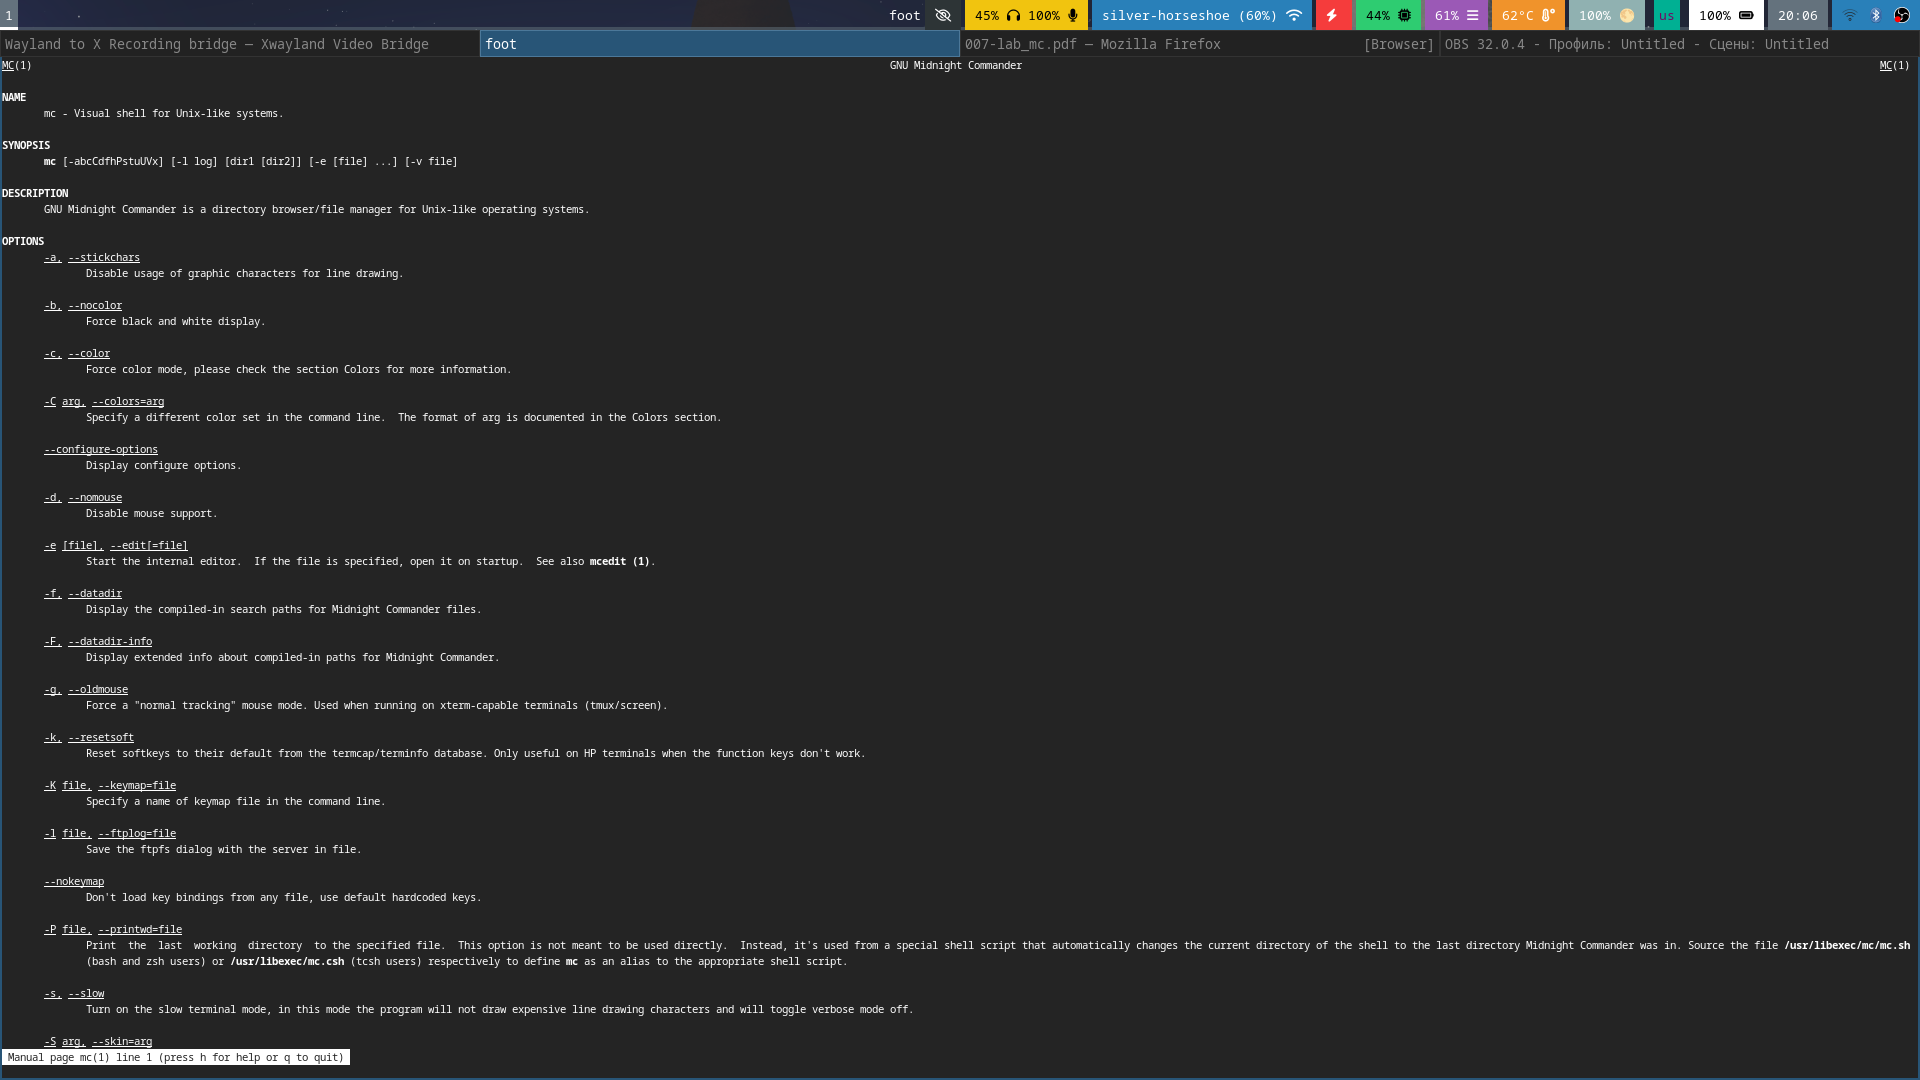
\includegraphics[keepaspectratio,alt={Вывод программы}]{image/Image1.png}}
- 2-ую задачу не имеет смысл расписывать так как все указано в
теоретической части - 3яя указана на видео.Получилось бы слишком много
скриншотов. Смотрим характеристики файла вроде прав доступа,содержания и
тп.
\pandocbounded{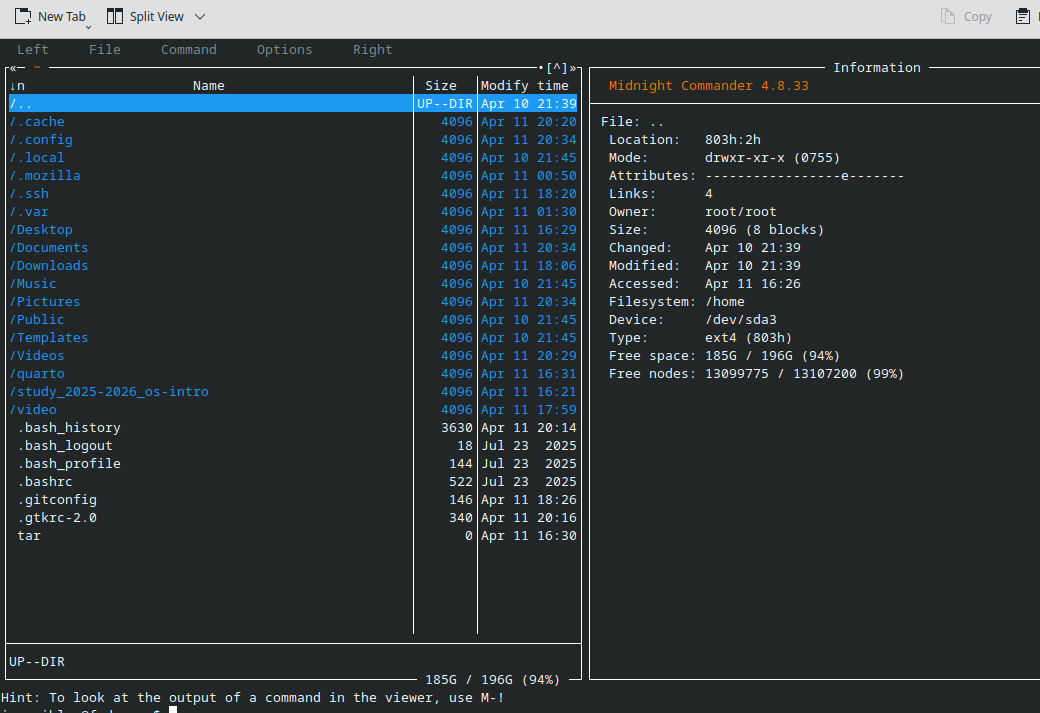
\includegraphics[keepaspectratio,alt={не знаю что писать}]{image/Image8.png}}
- Далее копируем все файлы.
\pandocbounded{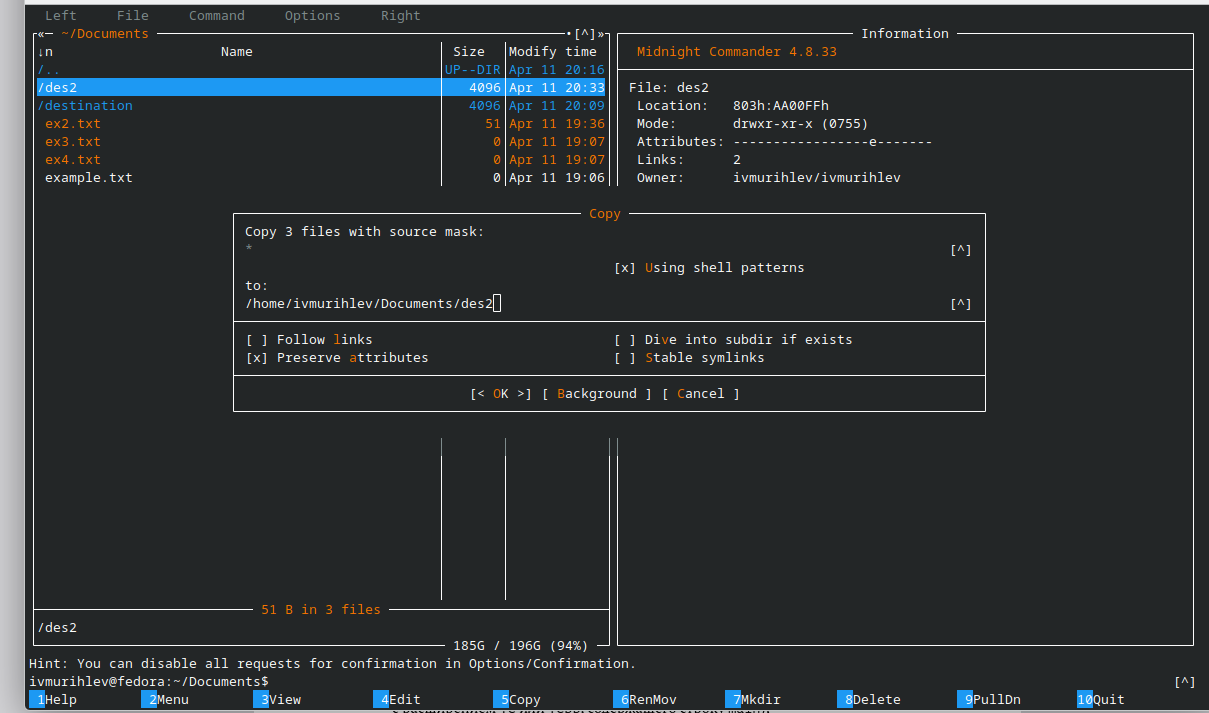
\includegraphics[keepaspectratio,alt={Копирование файлов в mc}]{image/Image7.png}}
\#\#\# В встроенном редакторе. - ПОсле создания файла открываем его в
редакторе.
\pandocbounded{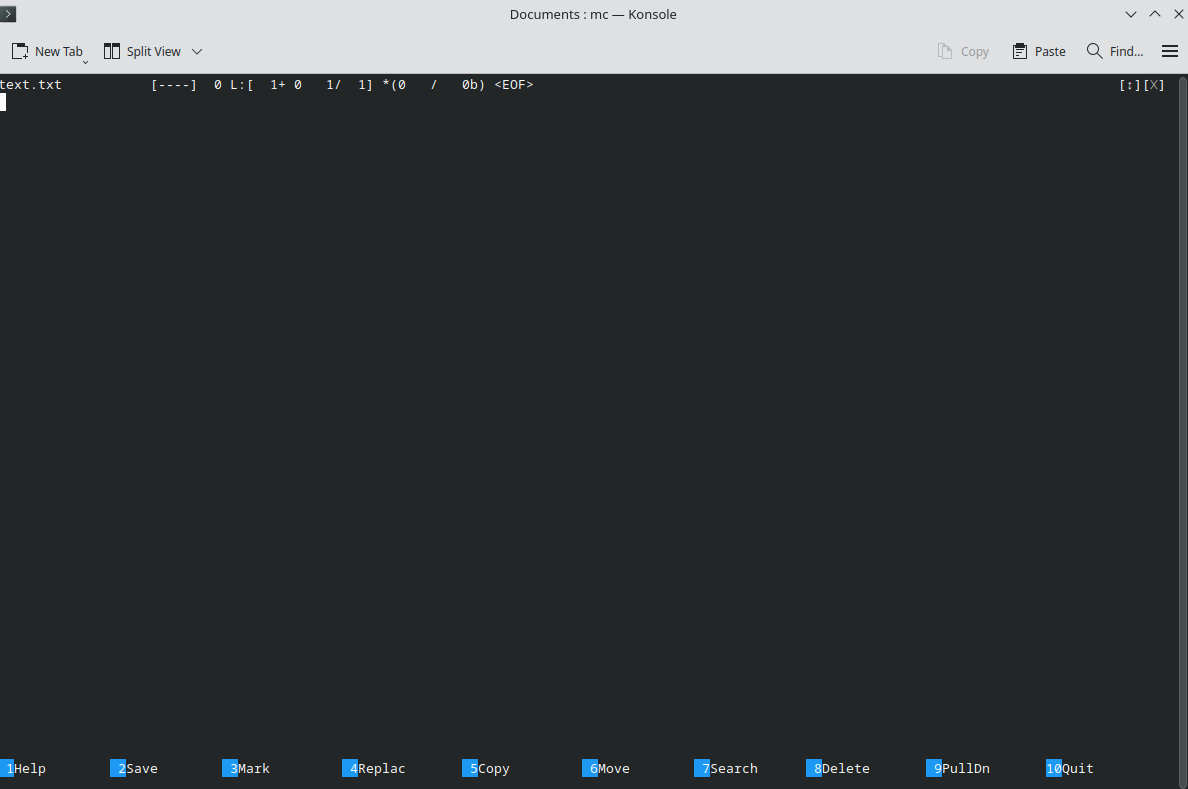
\includegraphics[keepaspectratio,alt={Пустой tetx.txt}]{image/Image9.png}}
- Затем вставлем текст
\pandocbounded{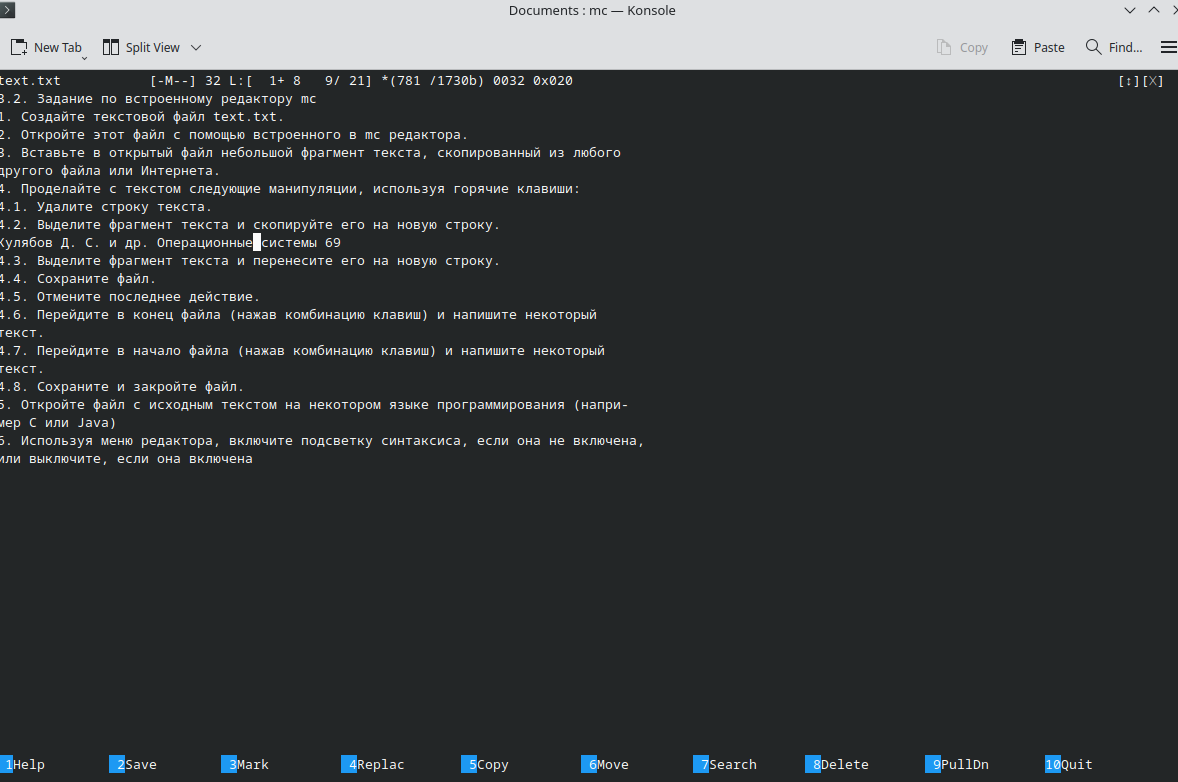
\includegraphics[keepaspectratio,alt={После вставки}]{image/Image10.png}}
- Дальнейшие задания представленны в видео ,так как демонстрируют
работу, которую долго описывать здесь. - 7 ctr + s - включение и
выключение подсветки синтаксиса.

\chapter{Выводы}\label{ux432ux44bux432ux43eux434ux44b}

Midnight commander предоставляет большой набор инструментов для работы с
ОС и оптимизации процессов навигации и поиска.\\
\# Контрольные вопросы 1. Режимы работы в mc: - Интерфейс командной
строки --- управление с помощью команд в терминале. - Графический режим
--- графический интерфейс с двумя панелями и меню. - Режим командной
строки внутри mc --- для выполнения команд напрямую.

\begin{enumerate}
\def\labelenumi{\arabic{enumi}.}
\setcounter{enumi}{1}
\tightlist
\item
  Операции с файлами, доступные через команды shell и меню:
\end{enumerate}

\begin{itemize}
\tightlist
\item
  Копирование файла (\texttt{F5} в меню или команда \texttt{cp}).
\item
  Удаление файла (\texttt{F8}).
\item
  Переименование (\texttt{F6}).
\item
  Создание новой папки (\texttt{F7})
\end{itemize}

\begin{enumerate}
\def\labelenumi{\arabic{enumi}.}
\setcounter{enumi}{2}
\tightlist
\item
  Структура меню левой (или правой) панели:
\end{enumerate}

\begin{itemize}
\tightlist
\item
  Обычно содержит отображение файлов и папок.
\item
  Можно настраивать отображение, фильтры, сортировку.
\item
  Команды позволяют управлять файлами (копировать, перемещать, удалять).
\end{itemize}

\begin{enumerate}
\def\labelenumi{\arabic{enumi}.}
\setcounter{enumi}{3}
\tightlist
\item
  Меню \enquote{Файл}:
\end{enumerate}

\begin{itemize}
\tightlist
\item
  Включает команды: Создать файл, Открыть, Сохранить, Выход.
\item
  Управление файлами и настройками открытия/сохранения.
\end{itemize}

\begin{enumerate}
\def\labelenumi{\arabic{enumi}.}
\setcounter{enumi}{4}
\tightlist
\item
  Меню \enquote{Команда}:
\end{enumerate}

\begin{itemize}
\tightlist
\item
  Выполнение системных команд, запуск скриптов.
\item
  Вставка команд, вызов внешних утилит.
\end{itemize}

\begin{enumerate}
\def\labelenumi{\arabic{enumi}.}
\setcounter{enumi}{5}
\tightlist
\item
  Меню \enquote{Настройки}:
\end{enumerate}

\begin{itemize}
\tightlist
\item
  Настройка внешнего вида, панели, цветовой схемы.
\item
  Конфигурация поведения mc.
\end{itemize}

\begin{enumerate}
\def\labelenumi{\arabic{enumi}.}
\setcounter{enumi}{6}
\tightlist
\item
  Встроенные команды mc:
\end{enumerate}

\begin{itemize}
\tightlist
\item
  Навигация по файлам
\item
  Обновление отображения..
\item
  Быстрый доступ к панели и меню.
\end{itemize}

\begin{enumerate}
\def\labelenumi{\arabic{enumi}.}
\setcounter{enumi}{7}
\tightlist
\item
  Команды встроенного редактора mc:
\end{enumerate}

\begin{itemize}
\tightlist
\item
  Вставка текста.
\item
  Режим поиска.
\item
  Отмена изменений.
\end{itemize}

\begin{enumerate}
\def\labelenumi{\arabic{enumi}.}
\setcounter{enumi}{8}
\tightlist
\item
  Средства для создания пользовательских меню:
\end{enumerate}

\begin{itemize}
\tightlist
\item
  Используются файлы конфигурации
\item
  Позволяют создавать свои пункты меню для быстрого доступа.
\end{itemize}

\begin{enumerate}
\def\labelenumi{\arabic{enumi}.}
\setcounter{enumi}{9}
\tightlist
\item
  Средства для выполнения действий над файлом:
\end{enumerate}

\begin{itemize}
\tightlist
\item
  Быстрые команды для копирования, перемещения, удаления.
\item
  Контекстное меню и горячие клавиши
\end{itemize}

\chapter*{Список
литературы}\label{ux441ux43fux438ux441ux43eux43a-ux43bux438ux442ux435ux440ux430ux442ux443ux440ux44b}
\addcontentsline{toc}{chapter}{Список литературы}

\printbibliography[heading=none]





\end{document}
